\documentclass[letterpaper, twoside]{article}
\topmargin= -0.4in
\textheight = +8.9in
\oddsidemargin = 0.05in
\evensidemargin = 0.05in
\textwidth = 6.5in

\usepackage{blindtext} % Package to generate dummy text throughout this template 

\usepackage[sc]{mathpazo} % Use the Palatino font
\usepackage[T1]{fontenc} % Use 8-bit encoding that has 256 glyphs
\linespread{1.05} % Line spacing - Palatino needs more space between lines
\usepackage{microtype} % Slightly tweak font spacing for aesthetics

\usepackage[english]{babel} % Language hyphenation and typographical rules

\usepackage[hmarginratio=1:1,top=32mm,columnsep=20pt]{geometry} % Document margins
\usepackage[hang, small,labelfont=bf,up,textfont=it,up]{caption} % Custom captions under/above floats in tables or figures
\usepackage{booktabs} % Horizontal rules in tables

\usepackage{lettrine} % The lettrine is the first enlarged letter at the beginning of the text

\usepackage{enumitem} % Customized lists
\setlist[itemize]{noitemsep} % Make itemize lists more compact

\usepackage{abstract} % Allows abstract customization
\renewcommand{\abstractnamefont}{\normalfont\bfseries} % Set the "Abstract" text to bold
\renewcommand{\abstracttextfont}{\normalfont\small\itshape} % Set the abstract itself to small italic text

\usepackage{titlesec} % Allows customization of titles
\renewcommand\thesection{\Roman{section}} % Roman numerals for the sections
\renewcommand\thesubsection{\roman{subsection}} % roman numerals for subsections
\titleformat{\section}[block]{\large\scshape\centering}{\thesection.}{1em}{} % Change the look of the section titles
\titleformat{\subsection}[block]{\large}{\thesubsection.}{1em}{} % Change the look of the section titles

\usepackage{fancyhdr} % Headers and footers
\pagestyle{fancy} % All pages have headers and footers
\fancyhead{} % Blank out the default header
\fancyfoot{} % Blank out the default footer
\fancyhead[C]{Variational generation of images by deep spatial architectures $\bullet$ June 2017 } % Custom header text
\fancyfoot[RO,LE]{\thepage} % Custom footer text

\usepackage{titling} % Customizing the title section
\usepackage{hyperref} % For hyperlinks in the PDF
\usepackage{amsmath}
\usepackage{tikz}
\usepackage{multicol}
\usepackage{float}
\usetikzlibrary{fit,positioning}

%----------------------------------------------------------------------------------------
%   TITLE SECTION
%----------------------------------------------------------------------------------------

\setlength{\droptitle}{-4\baselineskip} % Move the title up

\pretitle{\begin{center}\Huge\bfseries} % Article title formatting
\posttitle{\end{center}} % Article title closing formatting
\title{Variational generation of images by deep spatial architectures} % Article title
\author{%
\textsc{Arthur Viv\'e} \\% \thanks{A thank you or further information} \\[1ex] % Your name
Advisor: Yali Amit \\
Department of Statistics\\
University of Chicago \\ % Your institution
%\normalsize \href{mailto:john@smith.com}{john@smith.com} % Your email address
%\and % Uncomment if 2 authors are required, duplicate these 4 lines if more
%\textsc{Jane Smith}\thanks{Corresponding author} \\[1ex] % Second author's name
%\normalsize University of Utah \\ % Second author's institution
%\normalsize \href{mailto:jane@smith.com}{jane@smith.com} % Second author's email address
}
\date{\today} % Leave empty to omit a date
\renewcommand{\maketitlehookd}{%
\begin{abstract}
\noindent 
\end{abstract}
}

%----------------------------------------------------------------------------------------

\begin{document}


\noindent
\thispagestyle{empty}
\underline{\bf Master's Paper of the Department of Statistics, the
  University of Chicago}

\vspace{1.8in}
\begin{center}
{\bf\LARGE Variational generation of images by deep spatial architectures}
\\~\\


\vspace{1.4in}
{\Large Arthur Viv\'e}

\vspace{1.3in}
{\Large Advisor: Yali Amit \\}

\end{center}

\vspace{.6in}
{\Large Approved} ~\underline{~~~~~~~~~~~~~~~~~~
\small ~~~~~~~~~~~~~~~~~~~~~~~~~~~~}

\vspace{.2in}
{\Large Date} ~\underline{~~~~~~~~~~~~~~~~~~~~~~~~~~
{\small }~~~~~~~~~~~~~~~~~~~~~~~~~~~~~~~}

\vfill
\begin{center}{\large July-21, 2017}\end{center}

\newpage
\pagestyle{plain}
\setcounter{page}{1}

\begin{abstract}

\vspace{7mm}\noindent Given the recent successes of neural networks at generating images, we make an attempt to augment those models with high level information. More precisely, by introducing equivariance to a broad set of spatial transformation into the variational autoencoder \cite{Kingma.aevb}, we manage to better model natural images, leveraging the power of neural networks while staying in the statistical framework of variational inference. Such models allow us to sample credible candidates directly from the image distribution. Our models are based on dense neural networks and spatial transformer layers \cite{Jaderberg.stn}. We will show that by forcing one part of the network to be spatially invariant, and the other part to estimate the relevant pose in the image, we can generate high quality samples.
\end{abstract}

%\newpage
% \vspace{1.in}
\tableofcontents


\newpage

%%%%%%%%%%%%%%%%%%%%%%
% \section{Introduction}
%%%%%%%%%%%%%%%%%%%%%%


% Print the title
% \maketitle

%----------------------------------------------------------------------------------------
%   ARTICLE CONTENTS
%----------------------------------------------------------------------------------------
\section*{Introduction}
\addcontentsline{toc}{section}{Introduction}
    
  It is now well established that neural networks can successfully classify more than hundreds of classes with efficient architectures. This proves that such networks are able to learn non-linear representations of their inputs in spaces where different classes become linearly separable. Generative models, on the contrary, do not simply focus on the boundaries of different classes, but have to learn how to generate each of them. In this paper, we will show how to better generate images by designing an equivariant variational autoencoder. This network will insure equivariance by performing two tasks. First, it will learn a representation of the reference pose; second, it will learn a regression model for the spatial transformation. The combination of those two steps will allow us to achieve equivariance, as well as generating credible samples. We will also measure the quality of those samples by various methods.\\

  Because they are fundamentally latent variable models, those kinds of networks share properties associated with dimensionality reduction. Namely: denoising property, manifold learning and visualization when the number of latent variable is low. Such properties provide applications in data-driven restoration of images, deconvolutions, which are techniques which can be used in Archeology, Medical imaging, up to license plate deblurring.

  \subsection*{Related work}
    Latent variable models for images have had a long history in Statistics. In 1984, S. Geman and D. Geman \cite{Geman:1984:SRG:2286442.2286617} used Markov Random Fields for prior distribution on images and tried to restore degraded images by sampling from the posterior distribution by the introduction in the same paper of the Gibbs Sampler. More recently, Allassonière, Amit and Trouvé \cite{Allasson.statfram} defined a Bayesian framework to learn deformable template models, and an estimation method for this model based on the EM algorithm.\\

    More recent approaches to image generation and restoration comprise Kingman's Variational autoencoder \cite{Kingma.aevb} which combines deep auto-encoder and the framework of Variational inference, yielding efficient optimization procedure with a Bayesian regularization which do not need to be fine-tuned. In \cite{Goodfellow.gan}, Goodfellow and al. introduced Generative Adversarial Networks, which are based on a generator network and a discriminative network. The generator slowly learns how to generate credible samples from random noise while the discriminator learns how to distinguish between generated and genuine samples. This approach led to sharper images, but it is not clear how the noise really influences the generated image. Chen and al address this issue by the InfoGAN \cite{chen.infogan} which incorporates a maximization of the mutual information between the noise and the generated image in the GAN optimization process. This allows to map each component of the noisy code to an interpretable feature of the image (e.g. class, width, shape). A drawback of this architecture is the need to simultaneously optimize two objectives. Other "hybrid" approaches have been taken, mixing variational inference with GAN \cite{Mescheder.advvae} or mixing informational approach with variational autoencoders \cite{Zhao.infoVAE}. Even though those approaches do have theoretical justifications, they still need parameter selection which arise from their optimizing multiple objectives at the same time.\\

    Special layers have also been designed to encompass higher order information about images in deep neural networks. Starting from the now ubiquitous Convolutional layer \cite{lecun-gradientbased-learning-applied-1998}, different strategies have been taken to tackle other classes of transformation. Cohen and Welling \cite{cohen.groupequi} designed networks that smartly deal with equivariance for transformations that span finite groups. Another approach taken by Jaderberg and al \cite{Jaderberg.stn} is the Spatial transformer layer, which uses a small neural net to regress the parameters of a transformation and transforms the input according to those parameters. This kind of layer can be used either to learn equivariance or invariance \cite{Jaderberg.stn}.

\section{Important concepts}
  \subsection{Variational inference}
    Variational inference is a method to maximize likelihood in cases of intractable conditional distributions and large datasets, that avoid using Gibbs sampling or the EM algorithm. It is particularly suited for general latent variable models. More precisely, given a latent variable model such as \ref{latentvargraph}, where $z$ is unobserved but has a prior distribution, and $x$ is defined by its conditional distribution given $z$.
     We can derive the Evidence Lower BOund (ELBO \cite{Jordan:VarMethods}) of the loglikelihood:\\
    \begin{align}
    log p(x) & = log \int p(x, z)dz = log \int p(x, z) \frac{q(z|x)}{q(z|x)} dz = log E_{z\sim q(.|x)}[\frac{p(x, z)}{q(z|x)}] \\
             & \geq E_{z\sim q(.|x)}[log(p(x, z)) - log (q(z|x))] =: L(q)
    \end{align}
    By Jensen's inequality, where $q$ is the approximate posterior whose support should be larger than that of the true one.
    We can now easily link this lower bound to the Kullback-Leibler divergence between the prior distribution of $z$ and the approximate posterior distribution.
    \begin{align}
    L(q) = E_{z\sim q(.|x)}[log(p(x| z)p(z)) - log (q(z|x))] = -D_{KL} (q(z|x)||p(z)) + E_{z\sim q(.|x)}[log(p(x| z)]
    \end{align}
    Therefore, we can see that without knowing the posterior (or the joint) distribution, we can still optimize the likelihood by using an approximate posterior. Moreover, we can parametrize this $q$ and the conditional $p(x|z)$ so that we optimize the likelihood and find the parameters of the transformation between $z$ and $x$ while finding the best parameters for the approximate posterior. In its new form, the lower bound is composed of the divergence between $q$, the approximate posterior, and the prior on $z$, and a second part, which can be seen as a reconstruction error.\\

    As shown in \cite{Kingma.aevb}, another way to derive this bound is to explicitly expand the likelihood. This shows that the slack in the bound is taken by the KL-divergence between the approximate posterior and the true posterior. This shows a potential limitation of variational methods. First, there is no guarantee that a local maximum on the bound corresponds to a local maximum for the likelihood. Second, we have no guarantee that maximizing the lower bound will induce a small distance between the approximate and the true posterior. We are however optimizing over the divergence between the prior and the approximate posterior. But since we have quite a lot of data in our applications -this is partly why we are using variational methods after all-, the data is more likely to shape our posterior, and the prior will only have a small influence. This means that, once again, variational methods don't ensure the proximity between the actual posterior and the approximate one.



    \begin{figure}
    \centering
    \begin{tikzpicture}
    \tikzstyle{main}=[circle, minimum size = 10mm, thick, draw =black!80, node distance = 16mm]
    \tikzstyle{connect}=[-latex, thick]
    \tikzstyle{box}=[rectangle, draw=black!100]
      \node[main, fill = white!100] (z) {$z$};
      \node[main] (x) [right=of z] {$x$};
      \path (z) edge [connect] (x) ;
      \node[rectangle, inner sep=0mm, fit= (z) (x),label=below right:N, xshift=13mm] {};
    \end{tikzpicture}
    \caption{General Latent variable model.}
    \label{latentvargraph}
    \end{figure}



  \subsection{Variational autoencoder}
    Autoencoders are usually neural networks designed to regress their input on itself while keeping a bottleneck (a layer with a few units) in the network. The first part of the network, between the input and the bottleneck, is called the encoder, and the second part, between the bottleneck and the output (which we want to be close to the input), the decoder. The main idea is that the information about the input has to be compressed and carried by the small bottleneck and then decoded to reproduce the input. Those models share common features with dimensionality reduction techniques we discussed earlier and allow nonlinear transformations.\\

    In \cite{Kingma.aevb}, Kingma and Welling introduced variational inference for autoencoders to perform inference over continuous latent variables models. Their contribution is multiple. First, they use the neural nets to describe the approximate posterior $q(z|x)$ and the conditional distribution $p(x|z)$. Then, they reparametrize the approximate posterior to be able to sample from it and to get a less variable Monte-Carlo estimate of the reconstruction error (second term of the variational lower bound).\\

    The graphical model in this case is described in figure \ref{vaegraphmodel}. This assumes that we observe i.i.d. data $(x_i)$, and that for every sample, there is a corresponding unobserved $z_i$. To generate new data, it would suffice to draw independently new $z_i$'s from their prior distribution, and draw the $x_i$'s from the conditional. Our goal here is therefore to learn the conditional distribution. To do so, we parametrize the conditional distribution and the prior by $\theta$, while parametrizing the approximate posterior by $\phi$. We will therefore denote the prior $p_\theta(z)$, the conditional $p_\theta(x|z)$, and the approximate posterior $q_\phi(z|x)$. For the procedure to work, $p_\theta(z)$ and $p_\theta(x|z)$ need to be differentiable almost everywhere with respect to $\theta$, and $q_\phi(z|x)$ with respect to $\phi$, respectively. This assumption can be understood in terms of the actual neural network that will be used: $\theta$ and $\phi$ will be weights in the network. By this assumption, the score function, which is the lower bound $L$, will be differentiable with respect to the weights, which is mandatory if we hope to optimize it.\\

    Under this framework, the KL-divergence is often analytically tractable. This, however, is not the case of the reconstruction error which needs to be estimated by a Monte-Carlo estimator. Thanks to the reparametrization trick, they achieve this stable estimator:\\
    \begin{align}
    \hat L(\theta, \phi, x_i) = -D_{KL}(q_\phi(z|x_i)||p_\theta(z)) + \frac{1}{L} \sum_{j=1}^L log p_\theta(x_i | z_{i, j})
    \end{align}
    Where $x_i$ is an observed sample, $(z_{i, j})_{j\in \{1, ..., L\}}$ are independent samples from $q_\phi(.|x_i)$. Those samples are in fact obtained by the following reparametrization: $z_{i, j}= g_\phi(\epsilon_j, x)$, where $\epsilon_j$ are independent from the same fixed distribution from which it is easy to sample (e.g Gaussian).

    Thanks to this explicit score, we can design an appropriate network, and optimize it with the mini-batch version of the Auto-Encoding Variational Bayes algorithm, described in \cite{Kingma.aevb}. This algorithm iteratively considers a batch of samples in the dataset, samples noise $\epsilon$, creates the $z_i$'s, computes the gradient of the lower bound with respect to $\theta$ and $\phi$ thanks to the neural net structure, and update the corresponding estimates by a standard stochastic gradient ascent method (e.g. SGD, SGD with momentum, Adam). In this regard, we can consider the variational autoencoder as a classical autoencoder regularized by noise. \\

    Variational autoencoders have their limitations. Their most common drawback is that they tend to produce blurry samples when trained on images. The main reason is that the distance is pixelwise. This means that the model learns first how to match big areas, leaving the boundaries, which carry less weight in the cost function, poorly matched and blurry. Another drawback, which is less often discussed, is that when the latent space becomes too big, the quality of the samples deteriorates quite drastically. A possible interpretation lies in the generation process. Say we put a $d$-dimensional standard multivariate gaussian as a prior for $z$. The model has to learn how to match each point within the most probable region (i.e. the $d$-dimensional sphere of radius calibrated to match a chosen confidence probability) to a point in the distribution of the $x_i$'s. This mapping is learned through a finite number of examples. Each example is going to define a distribution $q_\phi(z|x)$ for the latent code, say, a gaussian with its center within the aforementioned sphere. It means that, in the latent space, the dataset covers a finite number of small $d$-dimensional spheres. Therefore, by the curse of dimensionality, when $d$ gets too large, there is little chance that picking a point from the prior distribution will lead to a reasonable candidate in the distribution of the $x_i$'s.
    We will see an example of this phenomenon in the experiments. This paper proposes a solution to address both of those issues.


    \begin{figure}
    \centering
    \begin{tikzpicture}
    \tikzstyle{main}=[circle, minimum size = 10mm, thick, draw =black!80, node distance = 16mm]
    \tikzstyle{connect}=[-latex, thick]
    \tikzstyle{box}=[rectangle, draw=black!100]
      \node[main] (theta) [right=of z]{$\theta$};
      \node[main] (z) {$z$};
      \node[main] (x) [below=of z] {$x$};
      \path
        (z) edge [connect] (x)
        (theta) edge [bend right, connect] (z)
        (theta) edge [bend right, connect] (x)
        (x) edge [bend left, connect, dashed] node {$\phi$} (z);
      \node[draw, fit=(z) (x),label=below right:N] {};
    \end{tikzpicture}
    \caption{Parametrization of the latent variable model.}
    \label{vaegraphmodel}
    \end{figure}

  \subsection{Invariance and equivariance}
        The main goal of this paper is to enhance the variational autoencoder with higher-level information to 1. produce sharper generated samples, regardless of the allocated dimension of the latent space and 2. disentangle the information encoded in the latent representation. The higher level information mainly consists of which equivariances the model should have. \\

        To define formally the notion of equivariance and invariance, let's denote $\mathcal{X}$ the space of our data point. If our model is a function $f$ from $\mathcal{X}$ to itself (e.g. a denoiser for images). Then $f$ is equivariant to a family of transformations $\mathcal{G} \subset \mathcal{X}^\mathcal{X}$ if: 
        $\forall g \in \mathcal{G}, f \circ g = g \circ f$.\\
        Similarly, if our model is a function $f$ from $\mathcal{X}$ to $\mathcal{Y}$ (not necessarly $\mathcal{X}$, e.g. a classifier), then $f$ is invariant to a family of transformations $\mathcal{G} \subset \mathcal{X}^\mathcal{X}$ if: 
        $\forall g \in \mathcal{G}, f \circ g = f$.\\
        For many types of signal, scale is a feature that should not change the meaning of the signal. For images, rotating, shearing or translating should not change the content of an image but rather express the pose of an object. For natural images, acquisition artifact such as brightness or contrast should also have little influence on the content of the image. Given this knowledge, it seems important to directly use those features as latent variables, and then use them to correct generated samples.\\

  \subsection{Transformer Layers}


    As we saw, several layers have been designed to allow neural networks to achieve equivariance or invariance to spatial transformations. In our case, since we aim at regressing the parameters, we choose Spatial Transformer layers \cite{Jaderberg.stn}. Those layers rely on two inputs, an image to transform, and the parameters of the transformation to use. The parameters are usually the output of a neural network themselves, so that there is a first network which regresses the parameters from the image, and then the layer applies the transformation. What is shown is that as long as the transformation is differentiable, the whole network can be trained end-to-end without having data about the pose of the objects in the images. The two transformations that are considered are the affine transformation (5 degrees of freedom: rotation, horizontal and vertical scale and translation or 6 degrees for the full $3\times 2$ matrix), and the thin plate splines transformation. The latter necessitates a sampling grid as parameters ($2 \times s^2$ degrees of freedom for a grid of size $s$). This grid defines the positions of the $s^2$ reference points in the original image. The positions of those reference points in the output image is fixed to be a squared grid of size $s$ such as $G_s = \{(\frac{i}{s}, \frac{j}{s}) | 0 \leq i,j \leq s\}$ the grid of size $s$ inscribed in $[0, 1] \times [0, 1]$. A thin plate spline is then regressed based on those $s^2$ data points. This regression yields a differentiable function from the 2D-plane to itself. The original grid which supports the input image passes through the regression function and produces a warped grid. The output is obtained by bilinear sampling of this warped grid on $G_m$, where $m$ is the number of desired pixels in the output (usually the same as the input).\\

    Based on this differentiable way to sample images, we will incorporate higher level information in the latent code and we will see how the choice of the type of transformation influences our model, what it allows and what it doesn't.

\section{Statistical Model}
    As generative model for images, we propose an adapted latent variable model shown in figure \ref{tvaegraphmodel}. We define a general purpose latent variable, denoted by $z$, as well as another hidden variable, $u$ which will specifically model the pose of the object in the image. Those two parameters determine the distribution of a single sample: $p_\theta(x|u,z)$. This relationship will be later on learned by a neural network. In order to decorrelate the pose estimation from the other factors of variability, we assume independence between the two type of hidden parameters, $z$ and $u$.
    Within this model our goal is to model the "true" distribution $p(x|z,u)$ by a decoder, function of $z$ and $u$. To do so, we can maximize a lower bound of the likelihood:

\begin{align}
log(p(x)) \geq L = - D_{KL}(q(z|x)||p(z)) - D_{KL}(q(u|x)||p(u)) + E_{(z, u)\sim q(.|x)}[log(p(x| z, u)]
\end{align}
 Where the KL-divergence breaks into two parts thanks to the independence assumption between $u$ and $z$ on the prior and on the approximate prior. We will see later in the experimentations to which extent this independence assumption holds.


    \begin{figure}[h]
    \centering
    \begin{tikzpicture}
    \tikzstyle{main}=[circle, minimum size = 10mm, thick, draw =black!80, node distance = 16mm]
    \tikzstyle{connect}=[-latex, thick]
    \tikzstyle{box}=[rectangle, draw=black!100]
      \node[main] (z) {$z$};
      \node[main] (u) [right=of z]{$u$};
      \node[main] (x) [below=of z] {$x$};
      \node[] (theta) [right=of u]{$\theta$};
      \path
        (z) edge [connect] (x)
        (u) edge [connect] (x)
        (theta) edge [bend right, connect] (z)
        (theta) edge [bend right, connect] (u)
        (theta) edge [bend left, connect] (x)
        (x) edge [bend left, connect, dashed] node {$\phi$} (z)
        (x) edge [bend left, connect, dashed] node {$\phi$} (u);
      \node[draw, fit=(z) (u) (x),label=below right:N] {};
    \end{tikzpicture}
    \caption{Parametrization of the latent variable model with pose $u$.}
    \label{tvaegraphmodel}
    \end{figure}

    In the experiments ran on the MNIST dataset \cite{mnistlecun} in \cite{Kingma.aevb}, it is shown that the latent code in the VAE contains information about the pose of an image, as well as other features such as the class, the width of the writing, the curvature of the shapes. By introducing this new parameter $u$, we hope to disentangle features that make sense and study more thoroughly the rest of the latent code, which can encompass information of heterogeneous nature.

\section{Subsequent Architectures}

Our goal being to generate new samples from the training data, we use three different architectures. The first one is the traditional Variational autoencoder (VAE) and does not have any spatial parameters. The second one (referred as T-VAE) estimates the parameters $z$ and $u$ as the VAE except that it makes use of the pose to transform the image after reconstruction by the autoencoder part. This architecture has been introduced by S. Song in \cite{Siyu:vae}. We stress the fact that, given $u$, the transformation is completely deterministic and non-learned. The rationale behind this architecture is the following: we hope that after convergence, the hidden layer behind the latent variables, denoted $y'$ will be the reference pose of the input. Meanwhile, the spatial layer will transform this image $y'$ to fit exactly the pose of the input. A priori, one drawback of this architecture is the fact that the input is directly linked to the hidden variables by a non-spatially equivariant network. For any pose the digit might be in, the encoder needs to extract the latent variables corresponding to the reference pose. Thus, the output $z$ of the encoder should be invariant to pose. Song showed in \cite{Siyu:vae} that the network is able to recover precisely the pose of the image in $u$, and that additionally, this network has good denoising property even when trained on noisy data.\\
To address this issue of learning invariance without any other tools than dense layers, we propose the third architecture (referred as DTVAE, for Double Transformer Variational AutoEncoder). In this new setting, the pose is estimated and directly corrected, yielding $y$, then the image $y$ passes through the traditional VAE and the appropriate spatial transformation is performed to the reconstructed $y'$ to recover the pose and get the final reconstruction $x'$. With this architecture, we hope to decouple information about the pose and other sources of variability.\\

The different network architectures are regrouped in figure \ref{architectures}. The notation are as follows, $x$ is the observed image, $y$ should be its upright version (for which the pose has been corrected), $x'$ is the reconstruction of $x$, and should be close to it after convergence, $y'$ is its upright counterpart. $u$ and $z$ are respectively the sampled pose and latent code associated with $x$.


    \begin{figure}[h]
    
    \begin{minipage}{.2\textwidth}
    
    \begin{tikzpicture}[cross/.style={path picture={ \draw[black] (path picture bounding box.south east) -- (path picture bounding box.north west) (path picture bounding box.south west) -- (path picture bounding box.north east);},
                                      node distance=5mm}]
    \tikzstyle{main}=[circle, minimum size = 10mm, thick, draw =black!80, node distance = 10mm]
    \tikzstyle{connect}=[-latex, thick]
    \tikzstyle{box}=[rectangle, draw=black!100]

      \node[] (x) {$x$};
      \node[draw] (hl1) [below=of x] {Neural network};
      \node[] (zpar) [below=of hl1]{$q_\phi(z|x)$};
      \node[draw,circle,cross, label=right:Sampler] (zsampler) [below=of zpar] {};
      \node[] (z) [below=of zsampler] {$z$};
      \node[draw] (hl2) [below=of z] {Neural network};
      \node[] (xprime) [below=of hl2] {$x'$};
      \path
        (x) edge [connect] (hl1)
        (hl1) edge [connect] (zpar)
        (zpar) edge [connect] (zsampler)
        (zsampler) edge [connect] (z)
        (z) edge [connect] (hl2)
        (hl2) edge [connect] (xprime);
    \end{tikzpicture}
    \end{minipage}
    \begin{minipage}{.33\textwidth}
    \begin{tikzpicture}[cross/.style={path picture={ \draw[black] (path picture bounding box.south east) -- (path picture bounding box.north west) (path picture bounding box.south west) -- (path picture bounding box.north east);},
                                      node distance=5mm}]
    \tikzstyle{main}=[circle, minimum size = 10mm, thick, draw =black!80, node distance = 10mm]
    \tikzstyle{connect}=[-latex, thick]
    \tikzstyle{box}=[rectangle, draw=black!100]

      \node[] (x) {$x$};
      \node[] (hl1) [below=of x] {Neural network};
      \node[] (hl1bis) [right=of hl1] {};
      \node[] (zpar) [below=of hl1]{$q_\phi(z|x)$};
      \node[] (upar) [right=of zpar]{$q_\phi(u|x)$};
      \node[draw,circle,cross] (zsampler) [below=of zpar] {};
      \node[draw,circle,cross] (usampler) [below=of upar] {};
      \node[] (z) [below=of zsampler] {$z$};
      \node[] (u) [below=of usampler] {$u$};
      \node[draw] (hl2) [below=of z] {Neural network};
      \node[] (yprime) [below=of hl2] {$y'$};
      \node[draw] (transformer) [below=of u] {Transformer};
      \node[] (xprime) [below=of transformer] {$x'$};
      \path
        (x) edge [connect] (hl1)
        (hl1) edge [connect] (zpar)
        (hl1bis) edge [connect] (upar)
        (zpar) edge [connect] (zsampler)
        (upar) edge [connect] (usampler)
        (zsampler) edge [connect] (z)
        (usampler) edge [connect] (u)
        (z) edge [connect] (hl2)
        (hl2) edge [connect] (yprime)
        (yprime) edge [bend left=80, looseness =1.5, connect] (xprime)
        (u) edge [connect] (transformer);
        % (transformer) edge [connect] (xprime)
      \node[draw, fit= (hl1) (hl1bis)] {};
      \node[fit= (zsampler) (usampler)] {Sampler};
      % \node[fit= (transformer), label=right:Transformer] {};
    \end{tikzpicture}
    \end{minipage}
    \begin{minipage}{.53\textwidth}
    \begin{tikzpicture}[cross/.style={path picture={ \draw[black] (path picture bounding box.south east) -- (path picture bounding box.north west) (path picture bounding box.south west) -- (path picture bounding box.north east);},
                                      node distance=5mm}]
    \tikzstyle{main}=[circle, minimum size = 10mm, thick, draw =black!80, node distance = 10mm]
    \tikzstyle{connect}=[-latex, thick]
    \tikzstyle{box}=[rectangle, draw=black!100]

      \node[] (x) {$x$};
      \node[draw] (transformer1) [below=of x] {Transformer$^{-1}$};
      \node[draw] (hl1bis) [left=of transformer1] {N. Net};
      \node[] (y) [right=of x, xshift=1 cm] {$y$};
      \node[draw] (hl1) [below=of y] {Neural Net};
      \node[] (zpar) [below=of hl1]{$q_\phi(z|x)$};
      \node[] (upar) [below=of hl1bis]{$q_\phi(u|x)$};
      \node[draw,circle,cross] (zsampler) [below=of zpar] {};
      \node[draw,circle,cross] (usampler) [below=of upar] {};
      \node[] (z) [below=of zsampler] {$z$};
      \node[] (u) [below=of usampler] {$u$};
      \node[draw] (hl2) [below=of z] {Neural net};
      \node[] (yprime) [below=of hl2] {$y'$};
      \node[draw] (transformer2) [right=of u, yshift=-2cm] {Transformer};
      \node[] (xprime) [below=of transformer2] {$x'$};
      \path
        (x) edge [connect, bend right=70, looseness=1.5] (y)
        (x) edge [connect] (hl1bis)
        % (transformer1) edge [connect] (y)
        (y) edge [connect] (hl1)
        (hl1) edge [connect] (zpar)
        (hl1bis) edge [connect] (upar)
        (zpar) edge [connect] (zsampler)
        (upar) edge [connect] (usampler)
        (zsampler) edge [connect] (z)
        (usampler) edge [connect] (u)
        (z) edge [connect] (hl2)
        (hl2) edge [connect] (yprime)
        (upar) edge [connect] (transformer1)
        (u) edge [connect] (transformer2)
        (yprime) edge [connect, bend right=70, looseness=1.2] (xprime);
        % (transformer2) edge [connect] (xprime)
      \node[fit=(upar), label=above right :Mode] {};
      % \node[fit= (transformer), label=right:Transformer] {};
    \end{tikzpicture}
    \end{minipage}
    \caption{Architectures of the different networks. Left: traditional Variational autoencoder (VAE). Middle: Transformer Variational Autoencoder (T-VAE). Right: Double Transformer Variational Autoencoder (DTVAE).}
    \label{architectures}
    \end{figure}

\section{Datasets and distributions}
We test those new architectures on the MNIST \cite{mnistlecun} dataset, which comprises 60,000 training samples and 10,000 testing samples of 28x28 pixels gray-scale images.
Each image represents a single handwritten digit between 0 and 9. We also tested on a variation of this dataset: rot-MNIST which comprises 1500 training samples of rotated samples of MNIST. The wide of rotation is the whole range of 360 degrees. \\

This dataset gives us information about the kind of distributions to use as priors and approximate posterior. Each image is going to be described as a vector of independent Bernoulli given the latent variables with vector of probability given by the output of the network. We should note that the marginal distribution of each pixel is close to a Beta(0.05, 0.25) -therefore putting most probability on 0 and 1-, but for the sake of simplicity, we stick to a Bernoulli distribution. As for the prior distributions, we assume a standard normal $N(0, I)$ for the latent code $z$. \\

For the spatial variables, we try different priors. The first one is equivalent to not putting a prior: we assume a uniform prior with approximate posterior distribution $q_\phi(u|x) = \delta_{f(x)}(u)$, where f(x) is the output of the encoder dedicated to $u$. This setup implies that the KL divergence on the spatial parameters is null, and that $u$ is a deterministic function of $x$.\\
If we want to put a more sensible prior, there is a few things to consider. First, $u$ has a physical meaning, and acts directly on the image through the transformer, on the contrary to z. This means in particular that we cannot simply put a normal prior with mean 0 and variance 1, because that would mean that the average transformation is the identity and that the variability is arbitrary. For the latent code $z$, it did not matter because the neural network itself can take care of setting the scale to a sensible value. This means that we have to estimate some parameters of the prior during the optimization process. Secondly, we have to pay attention to the covariance structure of $u$. If we look at the approximate posterior distribution of $u$ in cases of a uniform prior, there are correlations between components (up to 30\% for the affine mapping). This is actually quite natural; for the affine correlations, the matrix with 6 cells has an inner structure in terms of rotation $\psi$, shearing $(S_x, S_y)$, and translation $(T_x, T_y)$:\\

$M=
  \left[ {\begin{array}{ccc}
   a & b & c\\
   d & e & f\\
  \end{array} } \right]
 = 
  \left[ {\begin{array}{ccc}
   S_x cos \psi & -S_x sin \psi & S_x T_x\\
   S_y sin \psi & S_y cos \psi & S_y T_y\\
  \end{array} } \right]$

  Therefore, it might be better to put priors on those 5 interpretable variables than on the 6 cells of the matrix. A sensible prior in this case could be:\\
  $u = (\psi, log S_x, log S_y, T_x, T_y) \sim N(\nu^u, Diag(\tau_1^u, \tau_2^u, \tau_3^u, \tau_4^u, \tau_5^u))$\\

  The same problem arises for the thin plate splines. The 9 points of the grid we have been using previously are highly dependent. In the case of a rotation centered in the middle of the grid, all exterior points move together and are coupled in a non-linear fashion. This implies that using a gaussian prior (even with a dense covariance matrix) may fail to model the range of transformations. This is also a consequence of the assumption of independence between the class of a digit and its pose. If different priors were used on different classes, then using only a gaussian prior may be fine.\\

Those observations lead us to consider different priors, with varying number of parameters to be estimated during the optimization process. If we denote $id$ as the identity transform regardless of the transformation (affine or TPS), we can have the following priors:\\
$
u \sim N(id, Diag(\tau_1^u, ..., \tau_S^u)), \text{ with } (\tau_1^u, ..., \tau_S^u) \text{estimated} \\
u \sim N(\nu^u, Diag(\tau_1^u, ..., \tau_S^u)), \text{ with } \mu, (\tau_1^u, ..., \tau_S^u) \text{ estimated} \\
u \sim N(\nu^u, \Sigma), \text{ with } \mu, \Sigma \text{ estimated}\\
$

An easy way to fit those kinds of prior within the deep learning framework is to put a standard normal prior on $u'$ and define $u$ as the set of units of a dense layer without a non-linear activation. This implies that $u$ can be written $u = W u' + b$ with $W$ a weight matrix and b a bias. Now given that $u'$ follows a standard normal, we have $u$ distributed as a normal $N(b, WW^T)$. This parametrization allows us to constraint $b$ (if we want to center the prior on the identity) and $W$, whose shape is going to determine the shape of the covariance. If we want to fit a diagonal covariance, we set $u'$ to have the same dimension as $u$ and constrain $W$ to be of the form $Diag(\tau_1, ..., \tau_S)$. If we unconstrain $W$, this is equivalent to fitting a dense covariance matrix. Another trick allowed by this reparametrization is to choose the dimension of $u'$ to be lower than that of $u$. This controls the maximum rank of the covariance matrix: $\text{rank}(\Sigma) = \text{rank}(WW^T) = \text{rank}(W) \leq min(dim(u), dim(u')) = dim(u') $. By controlling the rank of the covariance matrix, we can control the degrees of freedom independently of the number of parameters for the transformation.\\

All those distributions can be reparametrized, which allows the autoencoder variational Bayes algorithm \cite{Kingma.aevb} to be used. 
For example, with normal distributions as priors we can have the following parameters.\\

$
\text{Priors:}\\
z \sim N(0, I)\\
u' \sim N(0, I)\\
\text{Approximate posteriors:}\\
 z | x \sim N(\mu^z(x), Diag(\sigma_1^z(x), ..., \sigma_D^z(x))\\
 u' | x \sim N(\mu^u(x), Diag(\sigma_1^u(x), ..., \sigma_S^u(x))\\
 \text{Conditional:}\\
 x_{i, j} \sim Bernoulli(x'_{i, j})
$\\
Where all the functions of x are outputs of the encoder part of the network, and $x'$ is the output of the decoder, deterministic function of $z$ and $u'$.
This yields the following KL-divergences, reconstruction error, and therefore lower bound:

\begin{align}
D_{KL}(q_\phi(z|x) || p(z)) = \frac{1}{2} \sum_{j=1}^D  -2 log (\sigma_j^z(x)) + (\mu^z(x))^2 + (\sigma_j^z(x))^2 - 1\\
D_{KL}(q_\phi(u'|x) || p(u')) = \frac{1}{2} \sum_{j=1}^D  -2 log (\sigma_j^u(x)) + (\mu^u(x))^2 + (\sigma_j^u(x))^2 - 1\\
% D_{KL}(q_\phi(u|x) || p(u)) = \frac{1}{2} \sum_{j=1}^S -2 log (\frac{\sigma_j^u(x)}{\tau_j^u}) + \frac{(\mu_j^u(x) - \nu_j^u)^2 + (\sigma_j^u(x))^2}{(\tau_j^u)^2} - 1\\
\frac{1}{L} \sum_{l=1}^L log p_\theta(x^n | z_{l}^i, u_{l}^{'i}) = \frac{1}{L} \sum_{l=1}^L \sum_{i, j} x_{i,j}^n log({x'}_{i, j}^{n, l}) + (1 - x_{i,j}^n) log(1 - {x'}_{i, j}^{n, l})\\
\hat L(x^n, \theta, \phi) = -D_{KL}(q_\phi(z|x^n) || p(z)) - D_{KL}(q_\phi(u'|x^n) || p(u')) + \frac{1}{L} \sum_{l=1}^L log p_\theta(x^n | z_{l}^i, u_{l}^{'i})
\end{align}

In all the experiments here, and as is done in \cite{Kingma.aevb}, we use $L=1$, and thus use a single draw from the approximate posterior per image to estimate the lower bound.

\section{Study of the general purpose latent code $z$}

In this section, we focus on the general purpose latent code and therefore do not put a prior on the spatial code $u$ (or equivalently, use a flat prior with a degenerate approximate posterior on it). This means that $u$ is a deterministic function of the image $x$. Also, since the focus here is not on modeling the distribution of the spatial code $u$, the digits are represented in their upright pose, which means that $u$ is set to the mean transformation over the training set. This allows different models which may have different internal representations of the digits to be compared.

\subsection{Dimension of the latent code}
\subsubsection{Reconstruction error}

The main goal of those experiments is to study how the architectures behave on MNIST when the number of latent variables and spatial variables changes. First, let's see if there is an ideal number of general purpose latent variables (i.e. $z$) for the MNIST dataset to fully understand the value of our models. From \ref{numlatent}, the optimal number of latent variables can be estimated to be around 25. As claimed by Kingma \cite{Kingma.aevb}, there is little overfitting as the dimensionality of the latent code grows. For the other models, we counted all the latent variables together ($dim(u) + dim(z)$), and used 6 degrees of freedom for the affine transformer, and 18 ($=2\times 3^2$) degrees of freedom for the thin plate spline (TPS) transformer. Based on this experiment, custom models achieve better reconstruction. Thus, even though part of the latent code is constrained to contain purely spatial information, the transformation step allows the network to fit more precisely the input, ending up with a lower reconstruction error. This difference is mainly significant for the TPS-TVAE and the DTVAE.\\

\begin{figure}[h]
\centering
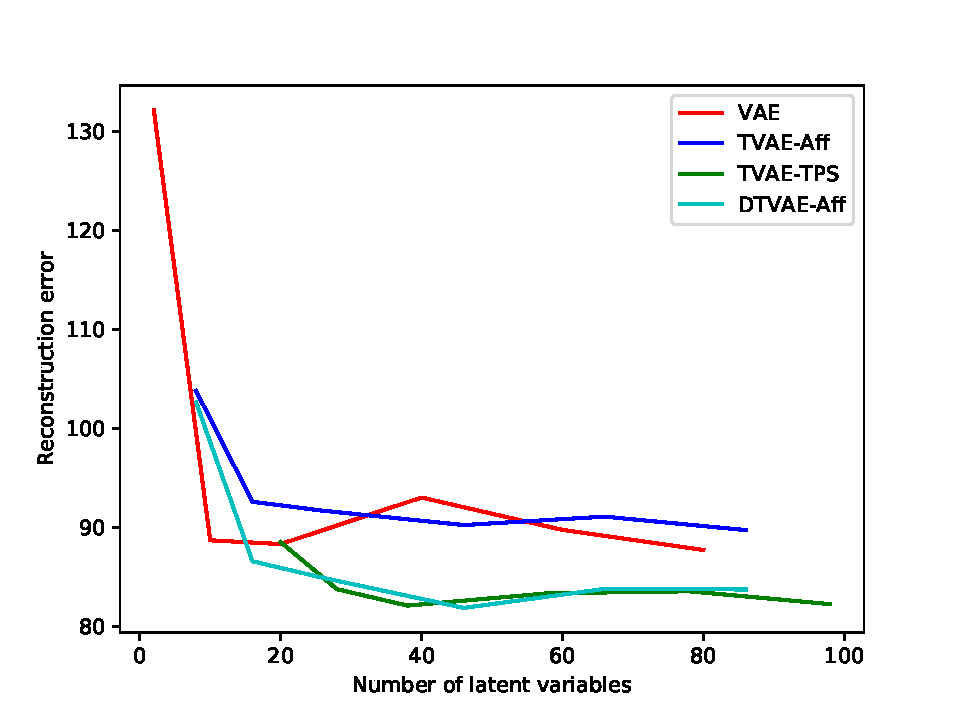
\includegraphics[scale=0.6]{num_latent.pdf}
\caption{Reconstruction error (second term of the likelihood) as a function of the dimensionality of the latent codes ($dim(z) + dim(u)$) for the standard Variational Autoencoder (Normal priors and approximate posterior, Bernoulli conditional) and derived transformer models -TVAE, DTVAE- (with deterministic relation between x and the pose $u$). The neural networks in the encoder and decoder are composed of 2 hidden layers of 256 units, and the localization network of the DTVAE is a single 128-unit layer.}
\label{numlatent}
\end{figure}

But this lower bound only gives information about the quality of the reconstruction and the appropriate number of the latent variables. What is also important for us is whether or not this model can produce credible samples.\\

  \subsubsection{Generating new upright samples}

We generate here samples from the three different models. Here, the focus is put on generating a new code $z$ and generating $x$ from $z$ (thanks to the decoder part of the network) and the average transformation observed on the training set for $u$. This means that we are not sampling the pose of the digit. We will discuss how to do that in a meaningful manner later. That is why, except for the VAE, all the samples are aligned in an upright direction.\\

From figure \ref{generatedcomparison}, we can witness the previously mentioned drawbacks of the VAE: the blurriness on generated samples, as well as the decaying quality of samples when the number of latent variables grows. This shows in particular that a high likelihood does not imply well generated images. As mentioned, the samples are in the upright direction for models which have a transformer layer, which means that the spatial regression part of each network is indeed working (as demonstrated in \cite{Siyu:vae}). We would like to point out the quality of the samples produced by the TVAE (middle column), which are sharper and whose quality is less affected by the number of latent variables.\\

\begin{figure}[H] 
\centering
\begin{minipage}{.33\textwidth}
\begin{flushleft}
\begin{tabular}{|@{}c@{}|}\hline
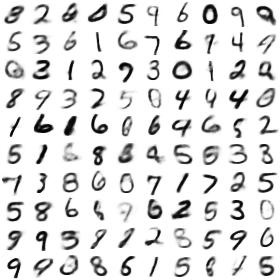
\includegraphics[scale=1]{manifold_119.jpg}\\ \hline
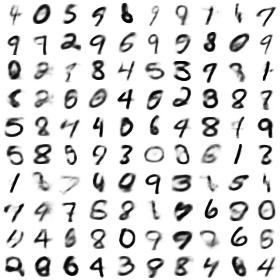
\includegraphics[scale=1]{manifold_120.jpg}\\\hline
\end{tabular}
\end{flushleft}
\end{minipage}%
\begin{minipage}{.33\textwidth}
\begin{tabular}{|@{}c@{}|}\hline
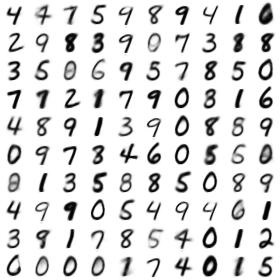
\includegraphics[scale=1]{manifold_126.jpg}\\ \hline
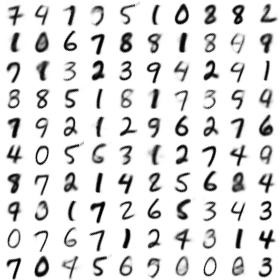
\includegraphics[scale=1]{manifold_127.jpg}\\ \hline
\end{tabular}
\end{minipage}

\caption{New samples generated by the models in their upright pose.Left: VAE. Right: TVAE with affine transformations. From top to bottom: respectively 10, 20 dimensions for the latent code $(z, u)$.\\ For each cell a latent code $z$ is drawn independently from the corresponding multivariate standard normal (For the TVAE, $u$ is set to the mean transformation over the training set). Both the encoder and the decoder part comprise 2 densely connected hidden layers of 256 hidden units.}
\label{generatedcomparison}
\end{figure}

\begin{figure}[H]
\centering
\begin{minipage}{.33\textwidth}
\begin{flushleft}
\begin{tabular}{|@{}c@{}|}\hline
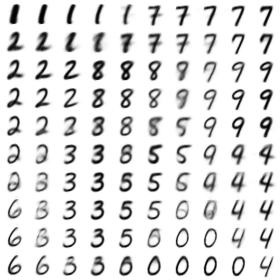
\includegraphics[scale=1]{manifold_86.jpg}\\ \hline
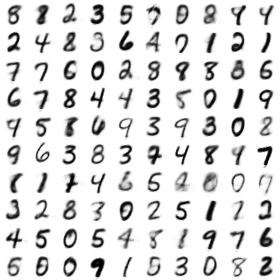
\includegraphics[scale=1]{manifold_87.jpg}\\ \hline
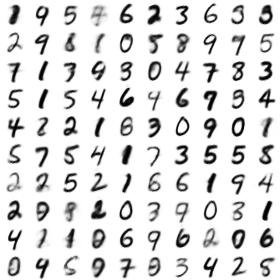
\includegraphics[scale=1]{manifold_88.jpg}\\\hline
\end{tabular}
\end{flushleft}
\end{minipage}%
\begin{minipage}{.33\textwidth}
\begin{tabular}{|@{}c@{}|}\hline
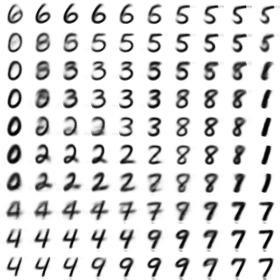
\includegraphics[scale=1]{manifold_132.jpg}\\ \hline
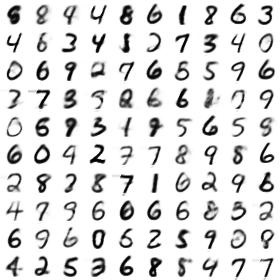
\includegraphics[scale=1]{manifold_133.jpg}\\ \hline
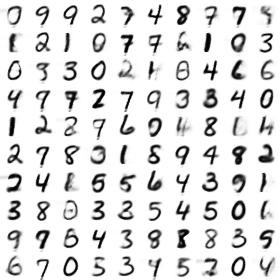
\includegraphics[scale=1]{manifold_134.jpg}\\ \hline
\end{tabular}
\end{minipage}

\caption{New samples generated by the models in their upright pose ($u$ set to the mean transformation).Left: TVAE with affine transformations. Right: DTVAE with affine transformations. From top to bottom: respectively 2, 10, 20 dimensions for the latent code $(z, u)$.\\ For each cell a latent code $z$ is drawn independently from the corresponding multivariate standard normal, except for the first line where the code varies continuously in 2 dimensions. $u$ is set to the identity. Both the encoder and the decoder part comprise 2 densely connected hidden layers of 256 hidden units, and the localization network (which predicts $u$) is a single dense layer of 128 units.}
\label{generatedcomparison2}
\end{figure}

  We designed the DTVAE in an attempt to uncouple spatial information from the rest of the variability in the image. It seems to perform as well as the TVAE in terms of generating performances.

  % This helps us develop an intuition about why the TVAE produces such sharp samples. On the contrary to the DTVAE, the TVAE learns to regress an image on its upright version ($x$ on $y'$). This means that the part of the encoder which is not regressing the spatial parameters is in charge of suppressing the pose, and learns spatial invariance. Our interpretation is that it acts like an inner data augmentation, which gives a natural way to the network to regularize itself. As we will discuss in the "Further developments" section, it could mean that enhancing this part of the network with layers designed to better achieve spatial invariance could lead to a great improvement.\\

  By using the TVAE, without using a prior on the pose $u$, we showed that we can fulfill all the properties of a classic autoencoder, while being able to generate new upright samples of better quality.

  \subsection{Latent code information}
    By the fixed machinery that we deployed, we know what the spatial variable $u$ contains, but did this reparametrization of the problem help disentangle the information in $z$?

    \subsubsection{Linear separation}
      To measure to which extent each algorithm provides a disentangled representation of the data, we feed the general purpose latent code $z$ to a linear Support Vector Machine. The results are gathered in table \ref{svmcompar}. In this test, the TVAE-Aff seems to do slightly better than the VAE, and the DTVAE is significantly superior to both. This trend is confirmed for a 20-dimensional latent code $z$, for which the gap between the VAE and the TVAE-Aff is wider. The DTVAE, however, does not improve between the two rounds. On the contrary, the TPS version of the TVAE greatly benefits from the higher dimension. It seems that the strategy deployed on the DTVAE to uncouple the information that is receiving the latent code in the TVAE worked: the information about the class is more linearly separable. Also, it seems that as dimension grows, the VAE behaves more and more like the standard PCA.\\


      \begin{table}[h]
        \centering
        \begin{tabular}{ | c || c | c | c |}
          \hline
          Input & Mean Accuracy (\%) & Standard deviation (\%) & Test accuracy\\ \hline \hline
          Raw MNIST ($28 \times 28 = 784$) & $91.19$ & $0.74$ & $91.80$\\ \hline \hline
          PCA ($8$) & $75.09$ & $1.32$ & $75.51$\\ \hline
          VAE ($8$) & $87.70$ & $0.93$ & $87.99$\\ \hline
          Affine-TVAE ($8$) & $89.30$ & $0.68$ & $88.39$\\ \hline
          TPS-TVAE ($8$) & $88.42$ & $0.58$ & $88.65$\\ \hline
          Affine-DTVAE ($8$) & $\mathbf{93.56}$ & $0.64$ & $\mathbf{93.87}$\\ \hline \hline
          PCA ($20$) & $85.62$ & $1.20$ & $86.52$\\ \hline
          VAE ($20$) & $85.77$ & $1.22$ & $86.45$\\ \hline
          Affine-TVAE ($20$) & $90.80$ & $0.66$ & $90.51$\\ \hline
          TPS-TVAE ($20$) & $\mathbf{94.65}$ & $0.46$& $\mathbf{94.48}$\\ \hline
          Affine-DTVAE ($20$) & $\mathbf{93.56}$ & $0.61$ & $\mathbf{94.17}$\\ \hline 

        \end{tabular}
        \caption{Accuracy of linear SVMs trained on latent codes produced by different models on MNIST (higher is better). Dimension of the input $z$ in parenthesis. To compute the mean accuracy and the standard deviation, we cross validated the models on the training set $9$ times.}
        \label{svmcompar}
      \end{table}

      % \begin{figure}[h]
      %   \centering
      %   \begin{minipage}{.5\textwidth}
      %   \centering
      %   \begin{tabular}{|@{}c@{}|}\hline
      %   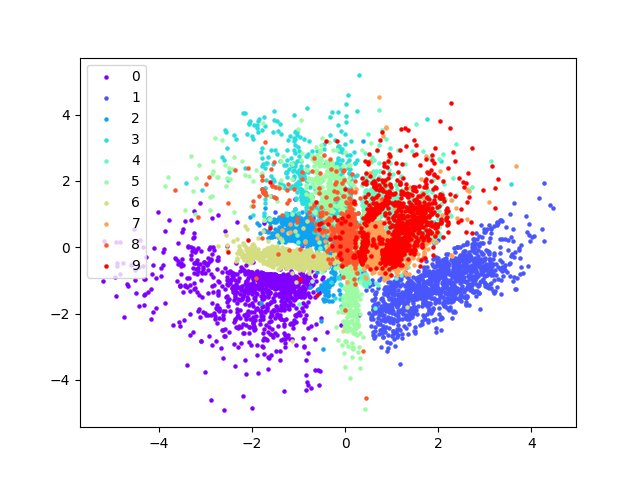
\includegraphics[scale=0.5]{dist_val_118.png}\\\hline
      %   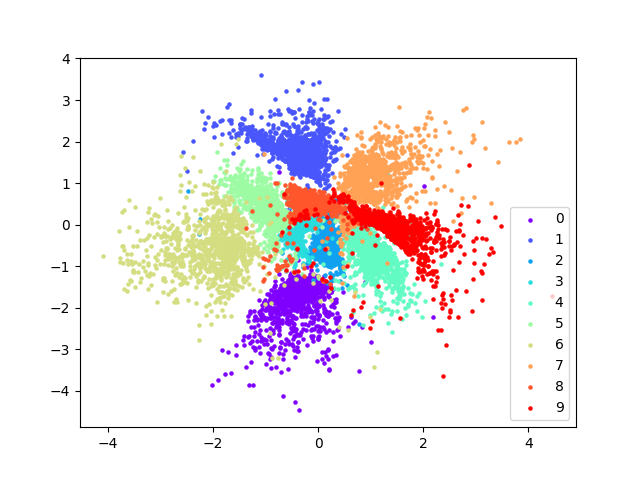
\includegraphics[scale=0.5]{dist_val_132.png}\\ \hline
      %   \end{tabular}
      %   \end{minipage}%
      %   \begin{minipage}{.5\textwidth}
      %   \centering
      %   \begin{tabular}{|@{}c@{}|}\hline
      %   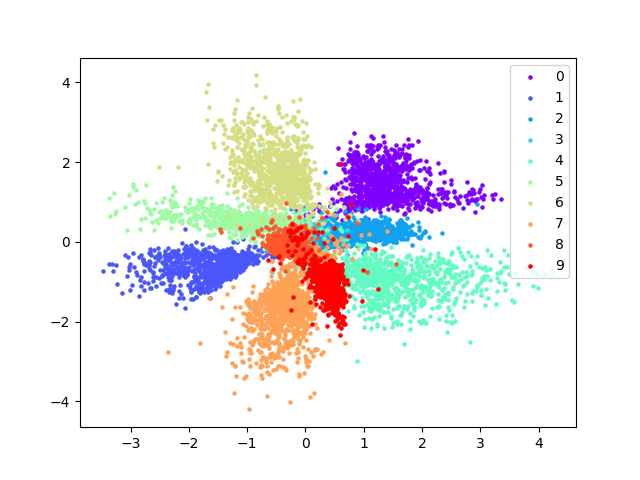
\includegraphics[scale=0.5]{dist_val_126.png}\\\hline
      %   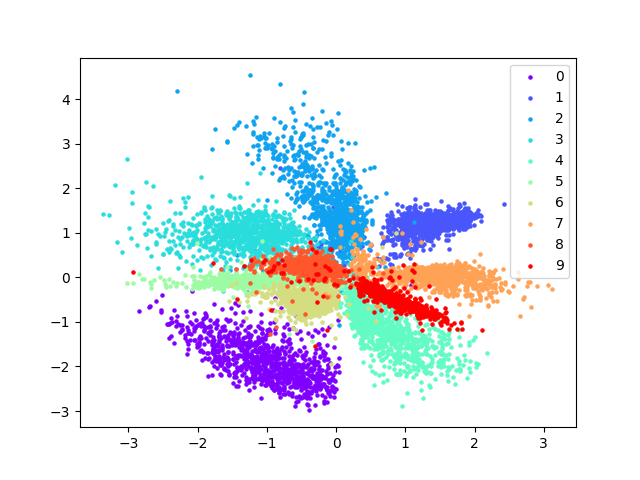
\includegraphics[scale=0.5]{dist_val_138.png}\\ \hline
      %   \end{tabular}
      %   \end{minipage}%
      %   \caption{Validation samples in a 2d-latent space.Top left: VAE.Top right: Affine TVAE, Top right: Affine TVAE. Bottom left: Affine DTVAE. Bottom right: TPS TVAE.}
      %   \label{2dlatent}
      % \end{figure}


      % From this, it seems hard to conclude anything more than that a more problem-specific architecture yields better features and therefore a better classification. In figure \ref{2dlatent}, we compare the different architectures in terms of the visualization they can offer. In 2D, except maybe for the VAE, is seems hard to distinguish if one model offers more separability than the others. From a generation perspective, it is important to understand that when we sample from a standard normal and hope to generate a well-formed digit, we pick a point in this ellipsoid. \\

\section{Study of the latent spatial variables}

  Since the TVAE shows nice properties, we will focus on it for the rest of the paper. As the transformer layer \cite{Jaderberg.stn} permits, we can use affine transformations as well as thin plate splines to model the deformations in the image. We can see from figure \ref{generatedafftps} that at least visually, the TPS seems to offer slightly sharper samples on average.\\

\begin{figure}[h]
\centering
\begin{minipage}{.5\textwidth}
\centering
\begin{tabular}{|@{}c@{}|}
\hline
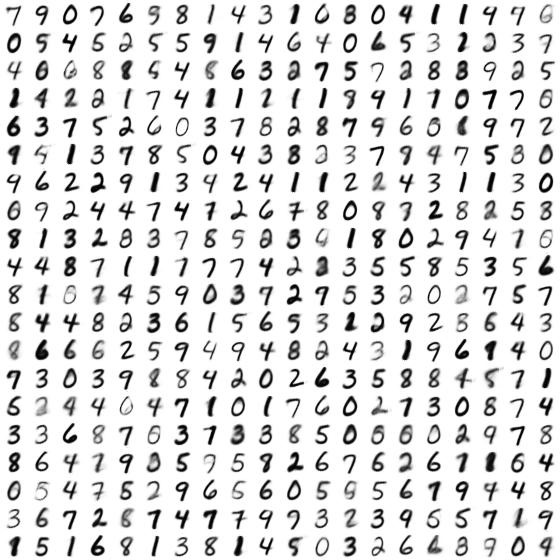
\includegraphics[scale=0.7]{manifold_28.jpg}\\\hline
\end{tabular}
\end{minipage}%
\begin{minipage}{.5\textwidth}
\centering
\begin{tabular}{|@{}c@{}|}
\hline
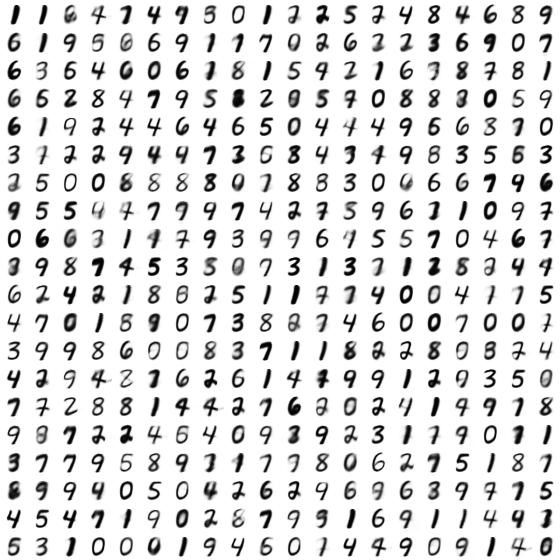
\includegraphics[scale=0.7]{manifold_39.jpg}\\\hline
\end{tabular}
\end{minipage}%
\caption{New samples generated by the models in the upright pose ($u$ set to the mean transformation).Left: TVAE with affine transformer. Right: TVAE with thin plate splines transformer. We use 30 dimensions for the latent code (left: $dim(z) = 24$, $dim(u) = 6$; right: $dim(z) = 12$, $dim(u) = 18$) .Each cell is drawn independently from the corresponding multivariate standard normal, while setting $u$ to its mean value on the training set (so that it behaves like the identity). No prior is put on $u$.}
\label{generatedafftps}
\end{figure}



  From figure \ref{generatedwithpose} onward, we use a prior on $u$ during training. In this figure, we make a comparison of different priors on the affine version of the TVAE. The first conclusion we can draw is that centering the prior on the identity mapping yields poor results. The expected posterior transformation is far from being the identity, therefore the procedure overestimated the prior variance, leading the samples with the sampled pose to be not satisfactory. If the prior mean is estimated, the prior on the 6 degrees of freedom of the affine transformation yields digits that are mainly sheared in the horizontal direction.\\

  \begin{figure}[H]
  \centering
  \begin{minipage}{.5\textwidth}
  \centering
  \begin{tabular}{|@{}c@{}|}
  \hline
  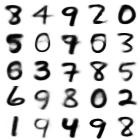
\includegraphics[scale=1]{manifold_ident_60.jpg}\\ \hline
  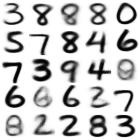
\includegraphics[scale=1]{manifold_ident_61.jpg}\\ \hline
  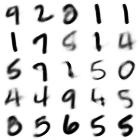
\includegraphics[scale=1]{manifold_ident_62.jpg}\\\hline
  \end{tabular}
  \end{minipage}%
  \begin{minipage}{.5\textwidth}
  \centering
  \begin{tabular}{|@{}c@{}|}
  \hline
  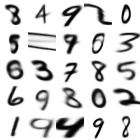
\includegraphics[scale=1]{manifold_sig_60.jpg}\\ \hline
  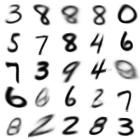
\includegraphics[scale=1]{manifold_sig_61.jpg}\\ \hline
  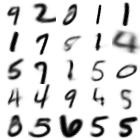
\includegraphics[scale=1]{manifold_sig_62.jpg}\\ \hline
  \end{tabular}
  \end{minipage}%
  \caption{Left: samples generated by a draw from the prior of the general latent code $z$ in their reference pose ($u$ set to the identity). Right: same samples than left transformed by a draw from the distribution on the spatial latent variable $u$. From top to bottom, different priors on $u$: normal prior with mean set to identity, estimated diagonal covariance on affine transformation with 6 d.o.f; normal prior with estimated mean, estimated diagonal covariance on affine transformation with 6 d.o.f; normal prior with estimated mean, estimated diagonal covariance on reparametrized affine transformation with 5 d.o.f.}
  \label{generatedwithpose} 
  \end{figure}

    Using the suggested prior on the reparametrized transformation with 5 degrees of freedom introduces a noticeable variation in rotation. We could argue that some digits do not seem to be in a "natural" pose. Our interpretation is that it is an artifact of the independence assumption between the pose $u$ and the class of the digit (contained in $z$). A visual way to understand this lies in figure \ref{generatedcomparison}. The long bar shared by the 7, the 1 and the 9 all have the same orientation. But the 1 is usually vertical in the dataset. This means that there is once again a co-adaptation between the general-purpose latent code $z$ and the pose $u$, and that this coadaptation is not done independently of the class.\\




\begin{figure}[H]
\centering
\begin{minipage}{.5\textwidth}
\centering
\begin{tabular}{|@{}c@{}|}
\hline
rank: 2\\
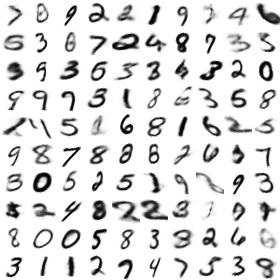
\includegraphics[scale=1]{manifold_sig_47.jpg}\\ \hline
rank: 4\\
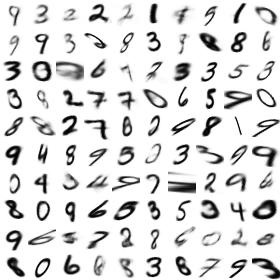
\includegraphics[scale=1]{manifold_sig_45.jpg}\\ \hline
rank: 6 ($=dim(u)$)\\
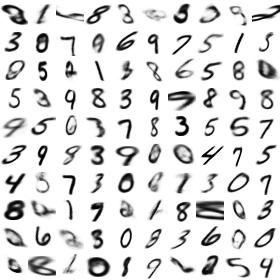
\includegraphics[scale=1]{manifold_sig_43.jpg}\\ \hline
\end{tabular}
\end{minipage}%
\begin{minipage}{.5\textwidth}
\centering
\begin{tabular}{|@{}c@{}|}
\hline
rank: 3\\
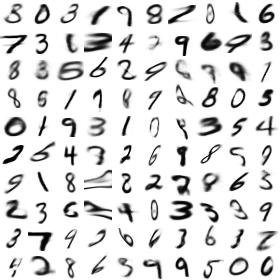
\includegraphics[scale=1]{manifold_sig_50.jpg}\\ \hline
rank: 9\\
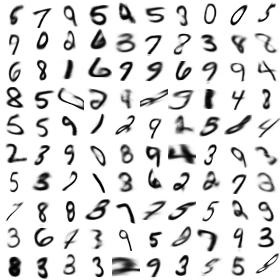
\includegraphics[scale=1]{manifold_sig_51.jpg}\\ \hline
rank: 18 ($=dim(u)$)\\
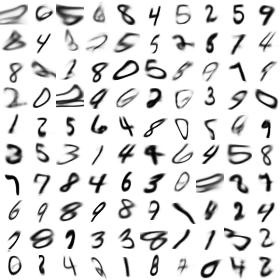
\includegraphics[scale=1]{manifold_sig_52.jpg}\\ \hline
\end{tabular}
\end{minipage}%
\caption{Samples from different models with an estimated full normal prior.Left: Affine TVAE (6-parameter transformation). Right: TPS TVAE (18-parameter transformation).}
\label{generatedfullprior} 
\end{figure}

  In both models, we can see that using a full covariance definitely increases the range of transformations allowed by the model. If we use the maximum rank, some samples seem to have extreme transformations that are not representative of the data. For a smaller dimension of $u'$, we seem to achieve a compromise between not too extreme transformations and a representatively broad variability in pose. Note that we could still develop more flexible priors by inserting a non-linear hidden layer between $u'$ and $u$, but it would of course be less interpretable and could only give us information about the relevant degree of freedom for the transformations.

\section{Optimization}
\subsection{Quality of the variational approximation}
  As discussed when we presented variational inference, the optimization of the lower bound does not offer a lot of guarantee that the approximate posterior is actually close to the true posterior. To experimentally check this, once the model fitted, we computed the marginal likelihood ($p(x)$) by Monte Carlo and compared it to the lower bound. As discussed, the difference between the two is the KL-divergence between the approximate posterior $q(z|x)$ and the true one $p(z|x)$.\\

  From Monte-Carlo sampling, experiments showed that the KL-divergence between the approximate and the true posterior is roughly equal to the KL-divergence between the approximate posterior and the prior, which is a quantity easily accessible and which we optimize during training. This is somewhat of a good compromise because without explicitly optimizing it, the approximate posterior is as close to the posterior as it is from the prior. But at the same time, we know from experience that the prior and the approximate posterior are very different because if we sample from the approximate posterior, we would always get very good samples (because those would be reconstruction from the dataset).


\subsection{Coadaptation within the network}
  An issue that can arise in those end-to-end learning models is that the different modules don't learn what we designed them to learn. In our case, one part of the network should regress the pose, and the other part should represent different kind of information in the image. It can happen that $z$ doesn't contain any information after convergence (i.e. it learned to produce only one template -usually a blurry 0-) which is bent by the code $u$ to match the input. Other poor local minima comprise the generation by the code $z$ of a downsampled version of the digit, see right of figure \ref{locmin}.

  \begin{figure}[h]
  \centering
  \begin{minipage}{.33\textwidth}
  \begin{tabular}{|@{}c@{}|}\hline
  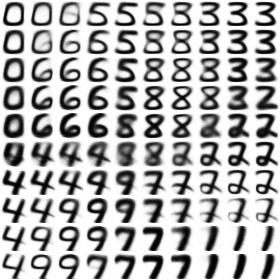
\includegraphics[scale=1]{manifold_good_min.jpg}\\ \hline
  \end{tabular}
  \end{minipage}%
  \begin{minipage}{.33\textwidth}
  \begin{tabular}{|@{}c@{}|}\hline
  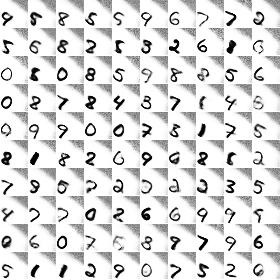
\includegraphics[scale=1]{manifold_bad_min.jpg}\\\hline
  \end{tabular}
  \end{minipage}%
  \caption{Different outputs of the decoder with transformation set to identity. Left: example a promising local minimum. Left: example of a poor local minimum.}
  \label{locmin}
  \end{figure}

    Usually, models that achieve a good reconstruction produce pre-transformation samples like the left of figure \ref{locmin}. In this case, the digit takes generally the whole space available and is very thick. This is interesting because it means that the transformation is able to downsample the digit and make it thinner according to the input. The internal representation has therefore a higher definition than the input. It is also important to note that more informative priors or adapted weights initialization centered on the identity transformation usually help avoid such poor local minima.

\section{Discussion}


      We showed how the TVAE and DTVAE were able to produce a general purpose latent code $z$ which has better properties in terms of linear separability and reconstruction abilities. For those use cases, there is no need to add a prior distribution on the spatial latent code $u$, and we can simply determine it deterministically. \\

      It is, however, important to note that the tasks of generation and reconstruction are opposed in this case. On the one hand, we would like the dataset to cover all the points in the latent space that are likely to be picked at generation time. That is to say, we would like the data to be scattered by the encoder in an ellipsoid centered on the origin in the latent space, so that when we sample from the prior, we always get a credible sample. But on the other hand, we would like the latent code $z$ to be very informative (e.g. of the class), so we would rather have clear margins between the classes in the latent space. We believe that this paradox fundamentally comes from a model misspecification. As we are trying to classify images, we implicitly make the assumption that there is some degree of discreteness in the latent code which is not allowed by our model. Several workarounds have been considered for this. A first option is to assume that the labels are known at generation and training time and we would fit the whole model conditionally on the labels. A more ambitious option would be to allow a fraction of the latent code $z$ to be discrete. Such parametrization usually allows to recover the classes in such a simple dataset \cite{chen.infogan}. However, the variational autoencoder does not allow discrete latent code because of the differentiability assumption. To work around this issue, an easy and approximate solution would be to penalize part of the code with an $L_1$ norm. Another solution would be to use the Gumbel-Softmax reparametrization \cite{JangCatReparam} which continuously approximate the categorical distribution through a temperature parameter.\\

      We also showed what priors could be put on the spatial latent code. By constraining the covariance in different ways and over different parametrization of the transformation, we can produce decent digits with their pose. Based on our experiments, priors with diagonal covariance on affine transformations produce samples that seem credible. \\

      Another issue linked to the lack of discreteness arises from those experiments. The fact that certain class have different range of transformation contradicts our independence assumption between the general latent code $z$ and the spatial latent code $u$. If we introduce discreteness in the model as we discussed earlier, either by a discrete code or by conditioning on the labels, we could define the transformation conditionally on the discrete code. For example, if different covariance matrices are estimated according to the class, generating a new sample could be done by 1. choosing (or sampling) the class of the digit to produce 2. sampling the latent code $z$ conditioned on the class, 3. sample the spatial code conditionally on the class.


\section{Future Work}

  As we previously discussed, further studies could be conducted on those models. First, to encode the general purpose latent code $z$, architectures specifically designed to produce invariance could be deployed such as Convolutionnal architectures \cite{lecun-gradientbased-learning-applied-1998} and Group-equivariant convolutional layers \cite{cohen.groupequi}. Second, another dataset should be used to confirm our conclusions. For the future we considered CIFAR-10 \cite{cifar10} and eventually SVHN \cite{svhn} as good benchmark datasets. Moreover, another feature to model may be discreteness in the dataset, as it seemed to lack in our model. This discreteness can be accounted for by an approximation of the categorical distribution by a continuous distribution \cite{JangCatReparam}. Finally, if we witnessed that our model produces less blurry samples than the vanilla variational autoencoder, it did not eliminate the root of this blur, which fundamentally comes from the pixelwise distance in the loss, or said differently, from the conditional distribution of the image. To correct that two paths could be considered. Either we specify a more appropriate conditional distribution (e.g. a Markov Random field \cite{Geman:1984:SRG:2286442.2286617} -even though those are usually difficult to sample from-), or we can deploy an adversarial strategy that may be less statistically justified, but has been shown to work in Generative adversarial networks \cite{Goodfellow.gan}.


\section*{Acknowledgments} 
\addcontentsline{toc}{section}{Acknowledgments}

  I would like to particularly thank Prof. Yali Amit for his precious advice and time, and more exactly for his ability to keep things simple when those neural networks allow the craziest things! I would also like to thank Siyu Song who very nicely got me up to speed with his work and allowed me to push it a little further. Let me thank also Yufei Feng and Jiajun Shen, with whom I had the opportunity to share my findings and who gave me feedback and help thanks to their experience, as well as their theoretical and practical knowledge of the field. Finally, I would like to thank Dr. Mei Wang for pushing her MS. students to do their best, so that they can be proud of their accomplishments.

\section*{Conclusion}
\addcontentsline{toc}{section}{Conclusion}

  In sum, we showed how to handle spatial information in the variational autoencoder, how it helped achieve better reconstruction as well as better generate new samples. This has been made possible by the careful design of the TVAE and DTVAE which take advantage of this high-level information. Thanks to those new models, we can achieve better unsupervised learning, representation and denoising, while staying in a statistically relevant framework. This paper more generally shows how to encompass higher level information in existing models. Similar treatment could have been given to generative adversarial networks \cite{Goodfellow.gan} for example, or even different types of variability for different signals.

%----------------------------------------------------------------------------------------
%   REFERENCE LIST
%----------------------------------------------------------------------------------------
\bibliographystyle{unsrt}
\bibliography{biblio}

\newpage
\appendix
\section{Neural networks architectures}

For the reproducibility of our results, we mention here the neural network architectures we used, as well as the hardware and software. \\
Hardware: Nvidia GTX 1080\\
Software: Lasagne 0.2.dev1 and Theano 0.8.2\\

Except when mentioned otherwise, the Neural Network block in figure \ref{architectures} consists of two hidden layers of 256 hidden units with rectified linear units as activation functions. The latent code mean is considered in the code as a Densely connected layer without activation, and the latent code log-standard deviation is also a Densely connected layer except that they are clipped to be more than $10^{-6}$. The used Transformer layer is the default one provided with Lasagne. To make the loss and gradients more stable, the output of the network is clipped to be within $[10^{-6}, 1 - 10^{-6}]$. If there is any instability with the spatial variable, it is possible to use an activation like $tanh$ or the sigmoid to limit their range, and scale them and shift them around the identity transformation.\\
Every presented model can converge in 50 epochs optimized by Adadelta (with default hyperparameters, see Lasagne documentation). In case of a bad local minimum, those models can be re-run.



\end{document}